\documentclass[prc]{revtex4}
\usepackage[dvips]{graphicx}
\usepackage{mathrsfs}
\usepackage{amsfonts}
\usepackage{lscape}

\usepackage{epic,eepic}
\usepackage{amsmath}
\usepackage{amssymb}
\usepackage[dvips]{epsfig}
\usepackage[T1]{fontenc}
\usepackage{hyperref}
\usepackage{bezier}
\usepackage{pstricks}
\usepackage{dcolumn}% Align table columns on decimal point
\usepackage{bm}% bold math
%\usepackage{braket}
\usepackage[dvips]{graphicx}
\usepackage{pst-plot}

\newcommand{\One}{\hat{\mathbf{1}}}
\newcommand{\eff}{\text{eff}}
\newcommand{\Heff}{\hat{H}_\text{eff}}
\newcommand{\Veff}{\hat{V}_\text{eff}}
\newcommand{\braket}[1]{\langle#1\rangle}
\newcommand{\Span}{\operatorname{sp}}
\newcommand{\tr}{\operatorname{trace}}
\newcommand{\diag}{\operatorname{diag}}
\newcommand{\bra}[1]{\left\langle #1 \right|}
\newcommand{\ket}[1]{\left| #1 \right\rangle}
\newcommand{\element}[3]
    {\bra{#1}#2\ket{#3}}

\newcommand{\normord}[1]{
    \left\{#1\right\}
}

\usepackage{amsmath}
\begin{document}

\title{Exercises FYS-KJM4480/9480, Second set, Week 36, deadline, September 8 3pm}
%\author{}
\maketitle
\subsection*{Exercise 3}
Consider three $N$-particle 
Slater determinants $|SD\rangle$, $|SD_i^j\rangle$ and $|SD_{ij}^{kl}\rangle$, where the notation means that 
Slater determinant $|SD_i^j\rangle$ differs from $|SD\rangle$ by one single-particle state, that is a single-particle
state $\psi_i$ is replaced by a single-particle state $\psi_j$. Similarly, the Slater determinant $|SD_{ij}^{kl}\rangle$
differs by two single-particle states from $|SD\rangle$.

We define thereafter a general onebody operator $\hat{F} = \sum_{i}^N\hat{f}(x_{i})$ and a general 
twobody operator $\hat{G}=\sum_{i>j}^N\hat{g}(x_{i},x_{j})$
with $g$ being invariant under the interchange of the coordinates of two particles.
The single-particle states $\psi_i$ are not necessarily eigenstates of $\hat{f}$.
\begin{enumerate}
\item[a)] Find the expectation values of 
\[
\langle SD |\hat{F}|SD\rangle,
\]
and
\[
\langle SD\hat{G}|SD\rangle.
\]
\item[b)] Find thereafter t
\[
\langle SD |\hat{F}|SD_i^j\rangle,
\]
and
\[
\langle SD\hat{G}|SD_i^j\rangle,
\]
and finally
\item[c)] find 
\[
\langle SD |\hat{F}|SD_{ij}^{kl}\rangle,
\]
and
\[
\langle SD\hat{G}|SD_{ij}^{kl}\rangle.
\]
What happens with the two-body operator if we have a transition probability  of the type
\[
\langle SD\hat{G}|SD_{ijk}^{lmn}\rangle,
\]
where the Slater determinant to the right of the operator differs by more than two single-particle states?
\end{enumerate}
\subsection*{Exercise 4}
\begin{enumerate}
\item[a)] Show that the density of particles with coordinates $\mathbf{x}$, is given by
\[
  n(\mathbf{x}) = N \int d\mathbf{x}_2 \dots d\mathbf{x}_N |\Psi_{AS}(\mathbf{x},\mathbf{x}_2,\dots,\mathbf{x}_N)|^2 
\]
can be written in terms of the single-particle states $\psi_k$ as 
\[
 n(\mathbf{x}) = \sum_k|\psi_k(\mathbf{x})|^2.
\]
\item[b)] Calculate the matrix elements (second quantization)
\[
\bra{\alpha_{1}\alpha_{2}}\hat{F}\ket{\alpha_{1}\alpha_{2}}
\]
and
\[
\bra{\alpha_{1}\alpha_{2}}\hat{G}\ket{\alpha_{1}\alpha_{2}}
\]
with
\[
\ket{\alpha_{1}\alpha_{2}}=a_{\alpha_{1}}^{\dagger}
a_{\alpha_{2}}^{\dagger}\ket{0} ,
\]
\[
\hat{F}=\sum_{\alpha\beta}\bra{\alpha}f\ket{\beta}
a_{\alpha}^{\dagger}a_{\beta}  ,
\]
\[
\bra{\alpha}f\ket{\beta}=\int \psi_{\alpha}^{*}(x)f(x)\psi_{\beta}(x)dx ,
\]
\[
\hat{G} = \frac{1}{2}\sum_{\alpha\beta\gamma\delta}
\bra{\alpha\beta}g\ket{\gamma\delta}
a_{\alpha}^{\dagger}a_{\beta}^{\dagger}a_{\delta}a_{\gamma} ,
\]
and
\[
\bra{\alpha\beta}g\ket{\gamma\delta}=
\int\int \psi_{\alpha}^{*}(x_{1})\psi_{\beta}^{*}(x_{2})g(x_{1},
x_{2})\psi_{\gamma}(x_{1})\psi_{\delta}(x_{2})dx_{1}dx_{2}
\]
Compare these results with those from exercise 1c).

\end{enumerate}
\end{document}


\subsection*{Exercise 3}
 \item 





\subsection*{Exercise 4}
We define the one-particle operator
\[
\hat{T}={\displaystyle
\sum_{\alpha\beta}}\bra{\alpha}t\ket{\beta}a_{\alpha}^
{\dagger}a_{\beta},
\]
and the two-particle operator
\[
\hat{V}=
\frac{1}{2}{\displaystyle
\sum_{\alpha\beta\gamma\delta}}\bra{\alpha\beta}
v\ket{\gamma\delta}a_{\alpha}^{\dagger}a_{\beta}^{\dagger}
a_{\delta}a_{\gamma}.
\]
We have defined a single-particle basis with quantum numbers given by the set of greek letters $\alpha,\beta,\gamma,\dots$
Show that the form of these operators remain unchanged under 
a transformation  of the single-particle basis given by 
\[
\ket{i}=\sum_{\lambda}\ket{\lambda}\left\langle \lambda | i \right\rangle,
\]
with $\lambda\in \left\{\alpha,\beta,\gamma,\dots\right\}$. 
Show also that
$a_{i}^{\dagger}a_{i}$ is the number operator
for  the orbital $\ket{i}$. 

Find also the expressions for the operators
$T$ and $V$ when $T$ is diagonal in the representation
$i$. 

Show also that the operator
\[
\hat{N}_p=
\frac{1}{2}{\displaystyle
\sum_{\alpha\neq \beta}}
a_{\alpha}^{\dagger}a_{\beta}^{\dagger}
a_{\beta}a_{\alpha},
\]
is an operator that represents the number of pairs. Can you rewrite the 
operators 
for $\hat{T}$ and $\hat{V}$ in terms of the above number operator?

\subsection*{Exercise 5}
Consider the Hamilton operator for a harmonic oscillator
($c=\hbar =1$)
\[
\hat{H}=\frac{1}{2m}p^{2}+\frac{1}{2}kx^{2},
\hspace{1cm}k=m\omega^{2}
\]
\begin{enumerate}
\item[a)] Define the operators
\[
a^{\dagger}=\frac{1}{\sqrt{2m\omega}}
(p+im\omega x),\hspace{1cm}a=\frac{1}{\sqrt{2m\omega}}
(p-im\omega x)
\]
and find the commutation relations for these operators by using the
corresponding relations for $p$ and $x$.
\item[b)] Show that
\[
H=\omega (a^{\dagger}a+\frac{1}{2})
\]
\item[c)] Show that if for a state $\ket{0}$ which satisfies
$\hat{H}\ket{0}=\frac{1}{2}\omega\ket{0}$, then we have
\[
\hat{H}\ket{n}=\hat{H}(a^{\dagger})^{n}\ket{0}=(n+\frac{1}{2})\omega\ket{n}
\]
\item[d)] Show that the state $\ket{0}$ from c), with the property
$a\ket{0}=0$, must exist.
\item[e)] Find the coordinate-space representation of 
$\ket{0}$ and explain how you would construct the wave functions for excited states based on this state.
\end{enumerate}
\subsection*{Exercise 6}
Starting with the Slater determinant 
\[
\Phi_{0}=\prod_{i=1}^{n}a_{\alpha_{i}}^{\dagger}\ket{0},
\]
use Wick's theorem to compute the normalization integral
$<\Phi_{0}|\Phi_{0}>$.


\subsection*{Exercise 7}
Compute the matrix element
\[
\bra{\alpha_{1}\alpha_{2}\alpha_{3}}G\ket{\alpha_{1}'
\alpha_{2}'\alpha_{3}'}
\]
using Wick's theorem and express the two-body operator
$G$ (from exercise 1) in the occupation number (second quantization) 
representation.

\subsection*{Exercise 8}
Write the two-particle operator
\[
G=\frac{1}{4}\sum_{\alpha\beta\gamma\delta}\bra{\alpha\beta}
g\ket{\gamma\delta}a_{\alpha}^{\dagger}a_{\beta}^{\dagger}
a_{\delta}a_{\gamma}
\]
in the quasi-particle representation for particles and holes
\[
b_{\alpha}^{\dagger}=\left\{\begin{array}{c}
a_{\alpha}^{\dagger}\\a_{\alpha}\end{array}\right.
\hspace{1cm}
b_{\alpha}=\left\{\begin{array}{cc}a_{\alpha}&\alpha>
\alpha_{F}\\
a_{\alpha}^{\dagger}&\alpha \leq \alpha_{F}
\end{array}\right.
\]
The two-body matrix elements are antisymmetric.


\subsection*{Exercise 9}
Use the results from exercise 8 and Wick's theorem to calculate 
\[
\bra{\beta_{1}\gamma_{1}^{-1}}G\ket{\beta_{2}\gamma_{2}^{-1}}
\]
You need to consider that case that
$\beta_{1}$ be equal
$\beta_{2}$ and that $\gamma_{1}$ be equal $\gamma_{2}$.


\subsection*{Exercise 10}
Show that the onebody part of the Hamiltonian
    \begin{equation*}
        \hat{H}_0 = \sum_{pq} \element{p}{\hat{h}_0}{q} a^\dagger_p a_q
    \end{equation*}
can be written, using standard annihilation and creation operators, in normal-ordered form as 
    \begin{align*}
        \hat{H}_0 &= \sum_{pq} \element{p}{\hat{h}_0}{q} a^\dagger_p a_q \nonumber \\
            &= \sum_{pq} \element{p}{\hat{h}_0}{q} \left\{a^\dagger_p a_q\right\} + 
                \delta_{pq\in i} \sum_{pq} \element{p}{\hat{h}_0}{q} \nonumber \\
            &= \sum_{pq} \element{p}{\hat{h}_0}{q} \left\{a^\dagger_p a_q\right\} +
                \sum_i \element{i}{\hat{h}_0}{i}
    \end{align*}
Explain the meaning of the various symbols. Which reference 
vacuum has been used?

\subsection*{Exercise 11}
Show that the twobody part of the Hamiltonian
    \begin{equation*}
        \hat{H}_I = \frac{1}{4} \sum_{pqrs} \element{pq}{\hat{v}}{rs} a^\dagger_p a^\dagger_q a_s  a_r
    \end{equation*}
can be written, using standard annihilation and creation operators, in normal-ordered form as 
    \begin{align*}
    \hat{H}_I &= \frac{1}{4} \sum_{pqrs} \element{pq}{\hat{v}}{rs} a^\dagger_p a^\dagger_q a_s  a_r \nonumber \\
        &= \frac{1}{4} \sum_{pqrs} \element{pq}{\hat{v}}{rs} \normord{a^\dagger_p a^\dagger_q a_s  a_r}
            + \sum_{pqi} \element{pi}{\hat{v}}{qi} \normord{a^\dagger_p a_q} 
            + \frac{1}{2} \sum_{ij} \element{ij}{\hat{v}}{ij}
    \end{align*}
Explain again the meaning of the various symbols.

     Derive the normal-ordered form of the threebody part of the Hamiltonian.
    \begin{align*}
    \hat{H}_3 &= \frac{1}{36} \sum_{\substack{
                        pqr \\
                        stu}}
                 \element{pqr}{\hat{v}_3}{stu} a^\dagger_p a^\dagger_q a^\dagger_r a_u a_t a_s\\
    \end{align*}
and specify the contributions to the twobody, onebody and the scalar part.


\subsection*{Exercise 12}
\begin{enumerate}
\item[a)] Place indices and write the algebraic expressions and discuss the physical meaning of the following diagrams:
\begin{figure}[hbtp]
\includegraphics[width=.4\textwidth]{fig2.ps}
\caption{Examples of diagrams.}
\end{figure}\newline
\item[b)] Can you find the  diagrammatic expression for $\bra{c}\hat{H}_I\ket{c}$ using the normal-ordered form from the previous exercise? 
\end{enumerate}
\subsection*{Exercise 13}
In this exercise  we will develop two simple models for studying the 
helium atom (with two electrons) and the beryllium atom with four electrons.

After having introduced the  Born-Oppenheimer approximation which effectively freezes out the nucleonic degrees
of freedom, the Hamiltonian for $N$ electrons takes the following form 
\[
  \hat{H} = \sum_{i=1}^{N} t(x_i) 
  - \sum_{i=1}^{N} k\frac{Ze^2}{r_i} + \sum_{i<j}^{N} \frac{ke^2}{r_{ij}},
\]
with $k=1.44$ eVnm. We will use atomic units, this means
that $\hbar=c=e=m_e=1$. The constant $k$ becomes also equal 1. 
The resulting energies have to be multiplied by $2\times 13.6$ eV
in order to obtain energies in eletronvolts.

 We can rewrite our Hamiltonians as
\begin{equation}
    \hat{H} = \hat{H_0} + \hat{H_I} 
    = \sum_{i=1}^{N}\hat{h}_0(x_i) + \sum_{i<j}^{N}\frac{1}{r_{ij}},
\label{H1H2}
\end{equation}
where  we have defined $r_{ij}=| {\bf r}_i-{\bf r}_j|$ and
$\hat{h}_0(x_i) =  \hat{t}(x_i) - \frac{Z}{r_i}$
The variable $x$ contains both the spatial coordinates and the spin values.
The first term of Eq.~(\ref{H1H2}), $H_0$, is the sum of the $N$
\emph{one-body} Hamiltonians $\hat{h}_0$. Each individual
Hamiltonian $\hat{h}_0$ contains the kinetic energy operator of an
electron and its potential energy due to the attraction of the
nucleus. The second term, $H_I$, is the sum of the $N(N-1)/2$
two-body interactions between each pair of electrons. Note that the double sum carries a restriction $i<j$.

As basis functions for our calculations we will use hydrogen-like single-particle functions.  This means the onebody operator is diagonal in this basis for states $i,j$ with quantum numbers $nlm_lsm_s$ with  
energies 
\[\langle i|\hat{h}_0| j\rangle =  -Z^2/2n^2\delta_{i,j}.\]  
The quantum number $n$ refers to the number of nodes 
of the wave function.  Observe that this expectation value is independent of spin.

We will in all calculations here restrict ourselves to only so-called $s$ -waves,
that is the orbital momentum $l$ is zero. We will also limit the quantum number $n$ to $n\le 3$.  It means that every $ns$ state can accomodate two electrons due to the spin degeneracy. This is illustrated in Fig.~\ref{fig:fighelium} here.
\begin{figure}[hbtp]
\vspace{1.0cm}
 \setlength{\unitlength}{1cm}
 \begin{picture}(15,4)
 \thicklines
\put(-0.6,1){\makebox(0,0){$1s$}}
\put(-0.6,2){\makebox(0,0){$2s$}}
\put(-0.6,3){\makebox(0,0){$3s$}}
% first 2-particle state
\put(0.8,1){\circle*{0.3}}
\put(1.7,1){\circle*{0.3}}
% second 2-particle state
\put(5.0,2){\circle*{0.3}}
\put(5.9,2){\circle*{0.3}}
% third 2-particle state
\put(9.2,1){\circle*{0.3}}
\put(10.1,3){\circle*{0.3}}
% fourth 2-particle state
\put(13.4,1){\circle*{0.3}}
\put(14.3,2){\circle*{0.3}}
\dashline[+1]{2.5}(0,1)(15,1)
\dashline[+1]{2.5}(0,2)(15,2)
\dashline[+1]{2.5}(0,3)(15,3)
 \end{picture}
\caption{Schematic plot of the possible single-particle levels with double degeneracy.
The filled circles indicate occupied particle states.
We show some possible two-particle states which can describe states in the helium atom. \label{fig:fighelium}}
\end{figure}

In the calculations you 
will need the Coulomb interaction with matrix elements
involving single-particle wave functions with $l=0$ only, the so-called $s$-waves.
We need only the radial part since the 
spherical harmonics for the $s$-waves are rather simple. We omit single-particle states with $l> 0$.
Our radial wave functions are
\[
R_{n0}(r)=\left(\frac{2Z}{n}\right)^{3/2}\sqrt{\frac{(n-1)!}{2n\times n!}}L_{n-1}^1(\frac{2Zr}{n})\exp{(-\frac{Zr}{n})},
\]
where $L_{n-1}^1(r)$ are the so-called Laguerre polynomials.
These wave functions can then be used to compute the direct part of the
Coulomb interaction
\[
\langle \alpha\beta| V| \gamma\delta\rangle = \int r_1^2dr_1 \int r_2^2dr_2R_{n_{\alpha}0}^*(r_1) R_{n_{\beta}0}^*(r_2) 
  \frac{1}{| {\bf r}_1-{\bf r}_2|}R_{n_{\gamma}0}(r_1)R_{n_{\delta}0}(r_2)
\]
Observe that this is only the radial integral and that the labels $\alpha\beta\gamma\delta$ refer only to the quantum numbers $nlm_l$, with $m_l$ the projection of the orbital momentum $l$. 
A similar expression can be found for the exchange part. Since we have restricted ourselves to only $s$-waves, these integrals are straightforward but tedious to calculate. As an addendum to this exercise we list all closed-form expressions for the relevant matrix elements. Note well that these matrix elements do not include spin. When setting up the final antisymmetrized matrix elements you need to consider the spin degrees of freedom as well. Please pay in particular special attention to the exchange part and the pertinent spin values of the single-particle states.  


We will also, for both helium and beryllium assume that the many-particle states we construct have always the same total spin projection $M_S=0$. This means that if we excite one or two particles from the ground state, the spins of the various single-particle states should always sum up to zero. 

\begin{enumerate}
\item[a)] We start with the helium atom and define our single-particle Hilbert space to consist of the single-particle orbits $1s$, $2s$ and $3s$, with their corresponding spin degeneracies, see Fig.~\ref{fig:fighelium}. 

Set up the ansatz for the ground state $|c\rangle = |\Phi_0\rangle$ in second 
quantization and define a table of single-particle states. Construct thereafter
all possible one-particle-one-hole excitations  $|\Phi_i^a\rangle$ where $i$ refer to levels below the Fermi level (define this level) and $a$ refers to particle states. Define particles and holes. The Slater determinants have to be written in terms of the respective creation and annihilation operators.
The states you construct should all have total spin projection $M_S=0$. 
Construct also all possible two-particle-two-hole states $|\Phi_{ij}^{ab}\rangle$  in a second quantization representation. 


\item[b)]  Define the Hamiltonian in a second-quantized form and use this to
compute the expectation value of the ground state (defining the so-called reference energy of the helium atom. 
Show that it is given by
\[
  E[\Phi_0] = \langle c | \hat{H}| c \rangle 
  = \sum_{i} \langle i | \hat{h}_0 | i\rangle+ \frac{1}{2}\sum_{ij}\left[\langle ij |\frac{1}{r}|ij\rangle-\langle ij |\frac{1}{r}|ji\rangle\right].
\]
Define properly the sums keeping in mind that the states $ij$ refer to all
quantum numbers $nlm_lsm_s$.
Use the values for the various matrix elements listed at the end of the exercise to find the value of $E$
as function of $Z=2$.
Be careful when you set up the matrix elements. Pay in particular attention to the spin values.
\item[c)]
Hereafter we will limit ourselves to a system which now contains only one-particle-one-hole
excitations beyond the chosen state $|c\rangle$.
Using the possible Slater determinants from exercise a) for the helium atom,   
compute also the expectation values (without inserting the explicit values for the matrix elements first) of 
\[
\langle c | \hat{H}| \Phi_i^a \rangle,
\] 
and 
\[
\langle \Phi_i^a | \hat{H}| \Phi_j^b \rangle.
\]
Represent these expectation values in a diagrammatic form, both for the onebody part and the two-body part of the Hamiltonian. 
 
Insert then the explicit values for the various matrix elements and 
set up the final Hamiltonian matrix and diagonalize it using for example
Octave, Matlab, Python, C++ or Fortran as programming tools.

Compare your results from those of exercise b) and comment your results. 
The exact energy with our Hamiltonian is $-2.9037$ atomic units for helium. This value is also close to the experimental energy.
\item[d)] We repeat exercises b) and c) but now for the beryllium atom.
Define the ansatz for $|c\rangle$ and limit yourself again to one-particle-one-hole excitations.   Compute the reference energy 
$\langle c | \hat{H}| c \rangle $ for $Z=4$.  
Thereafter you will need to set up the appropriate Hamiltonian matrix
which involves also one-particle-one-hole excitations. Diagonalize this matrix
and compare your eigenvalues with $\langle c | \hat{H}| c \rangle$ for $Z=4$ and comment your results. 
The exact energy with our Hamiltonian is $-14.6674$ atomic units for beryllium. This value is again close to the experimental energy.
\end{enumerate}

We conclude by listing in Table \ref{tab:mtxlisting} the matrix elements for the radial integrals to be used for the direct part and the exchange part. Note again that these integrals do not include spin. 
\begin{table}[htbp]
\caption{Closed form expressions for the Coulomb matrix elements. The nomenclature is $1=1s$, $2=2s$ and $3=3s$, with no
spin degrees of freedom. \label{tab:mtxlisting}}
\begin{tabular} {|cr|cr|} \hline 
$\langle 11|V|11\rangle  =$& $ (5Z)/8 $ &$\langle 11|V|12\rangle  =$& $ (4096\sqrt{2}Z)/64827$ \\
$\langle 11|V|13\rangle  =$& $ (1269\sqrt{3}Z)/50000$ &$\langle 11|V|21\rangle  =$& $ (4096\sqrt{2}Z)/64827$ \\
$\langle 11|V|22\rangle  =$& $ (16Z)/729$ & $\langle 11|V|23\rangle  =$& $ (110592\sqrt{6}Z)/24137569$ \\
$\langle 11|V|31\rangle  =$& $ (1269\sqrt{3}Z)/50000$ &$\langle 11|V|32\rangle  =$& $ (110592\sqrt{6}Z)/24137569$ \\
$\langle 11|V|33\rangle  =$& $ (189Z)/32768$ & $\langle 12|V|11\rangle  =$& $ (4096\sqrt{2}Z)/64827$ \\
$\langle 12|V|12\rangle  =$& $ (17Z)/81$ &$\langle 12|V|13\rangle  =$& $ (1555918848\sqrt{6}Z)/75429903125$ \\
$\langle 12|V|21\rangle  =$& $ (16Z)/729$ &$\langle 12|V|22\rangle  =$& $ (512\sqrt{2}Z)/84375$ \\
$\langle 12|V|23\rangle  =$& $ (2160\sqrt{3}Z)/823543$ &$\langle 12|V|31\rangle  =$& $ (110592\sqrt{6}Z)/24137569$ \\
$\langle 12|V|32\rangle  =$& $ (29943\sqrt{3}Z)/13176688$ &$\langle 12|V|33\rangle  =$& $ (1216512\sqrt{2}Z)/815730721$ \\
$\langle 13|V|11\rangle  =$& $ (1269\sqrt{3}Z)/50000$ &$\langle 13|V|12\rangle  =$& $ (1555918848\sqrt{6}Z)/75429903125$ \\
$\langle 13|V|13\rangle  =$& $ (815Z)/8192$ & $\langle 13|V|21\rangle  =$& $ (110592\sqrt{6}Z)/24137569$ \\
$\langle 13|V|22\rangle  =$& $ (2160\sqrt{3}Z)/823543$ & $\langle 13|V|23\rangle  =$& $ (37826560\sqrt{2}Z)/22024729467$ \\
$\langle 13|V|31\rangle  =$& $ (189Z)/32768$ & $\langle 13|V|32\rangle  =$& $ (1216512\sqrt{2}Z)/815730721$ \\
$\langle 13|V|33\rangle  =$& $ (617Z)/(314928\sqrt{3})$ &$\langle 21|V|11\rangle  =$& $ (4096\sqrt{2}Z)/64827$ \\
$\langle 21|V|12\rangle  =$& $ (16Z)/729$ & $\langle 21|V|13\rangle  =$& $ (110592\sqrt{6}Z)/24137569$ \\
$\langle 21|V|21\rangle  =$& $ (17Z)/81$ & $\langle 21|V|22\rangle  =$& $ (512\sqrt{2}Z)/84375$ \\
$\langle 21|V|23\rangle  =$& $ (29943\sqrt{3}Z)/13176688$ & $\langle 21|V|31\rangle  =$& $ (1555918848\sqrt{6}Z)/75429903125$ \\
$\langle 21|V|32\rangle  =$& $ (2160\sqrt{3}Z)/823543$ & $\langle 21|V|33\rangle  =$& $ (1216512\sqrt{2}Z)/815730721$ \\
$\langle 22|V|11\rangle  =$& $ (16Z)/729$ & $\langle 22|V|12\rangle  =$& $ (512\sqrt{2}Z)/84375$ \\
$\langle 22|V|13\rangle  =$& $ (2160\sqrt{3}Z)/823543$ & $\langle 22|V|21\rangle  =$& $ (512\sqrt{2}Z)/84375$ \\
$\langle 22|V|22\rangle  =$& $ (77Z)/512$ & $\langle 22|V|23\rangle  =$& $ (5870679552\sqrt{6}Z)/669871503125$ \\
$\langle 22|V|31\rangle  =$& $ (2160\sqrt{3}Z)/823543$ & $\langle 22|V|32\rangle  =$& $ (5870679552\sqrt{6}Z)/669871503125$ \\
$\langle 22|V|33\rangle  =$& $ (73008Z)/9765625$ & $\langle 23|V|11\rangle  =$& $ (110592\sqrt{6}Z)/24137569$ \\
$\langle 23|V|12\rangle  =$& $ (2160\sqrt{3}Z)/823543$ & $\langle 23|V|13\rangle  =$& $ (37826560\sqrt{2}Z)/22024729467$ \\
$\langle 23|V|21\rangle  =$& $ (29943\sqrt{3}Z)/13176688$ & $\langle 23|V|22\rangle  =$& $ (5870679552\sqrt{6}Z)/669871503125$ \\
$\langle 23|V|23\rangle  =$& $ (32857Z)/390625$ & $\langle 23|V|31\rangle  =$& $ (1216512\sqrt{2}Z)/815730721$ \\
$\langle 23|V|32\rangle  =$& $ (73008Z)/9765625$ & $\langle 23|V|33\rangle  =$& $ (6890942464\sqrt{2/3}Z)/1210689028125$ \\
$\langle 31|V|11\rangle  =$& $ (1269\sqrt{3}Z)/50000$ & $\langle 31|V|12\rangle  =$& $ (110592\sqrt{6}Z)/24137569$ \\
$\langle 31|V|13\rangle  =$& $ (189Z)/32768$ & $\langle 31|V|21\rangle  =$& $ (1555918848\sqrt{6}Z)/75429903125$ \\
$\langle 31|V|22\rangle  =$& $ (2160\sqrt{3}Z)/823543$ & $\langle 31|V|23\rangle  =$& $ (1216512\sqrt{2}Z)/815730721$ \\
$\langle 31|V|31\rangle  =$& $ (815Z)/8192$ & $\langle 31|V|32\rangle  =$& $ (37826560\sqrt{2}Z)/22024729467$ \\
$\langle 31|V|33\rangle  =$& $ (617Z)/(314928\sqrt{3})$ & $\langle 32|V|11\rangle  =$& $ (110592\sqrt{6}Z)/24137569$ \\
$\langle 32|V|12\rangle  =$& $ (29943\sqrt{3}Z)/13176688$ & $\langle 32|V|13\rangle  =$& $ (1216512\sqrt{2}Z)/815730721$ \\
$\langle 32|V|21\rangle  =$& $ (2160\sqrt{3}Z)/823543$ & $\langle 32|V|22\rangle  =$& $ (5870679552\sqrt{6}Z)/669871503125$ \\
$\langle 32|V|23\rangle  =$& $ (73008Z)/9765625$ & $\langle 32|V|31\rangle  =$& $ (37826560\sqrt{2}Z)/22024729467$ \\
$\langle 32|V|32\rangle  =$& $ (32857Z)/390625$ & $\langle 32|V|33\rangle  =$& $ (6890942464\sqrt{2/3}Z)/1210689028125$ \\
$\langle 33|V|11\rangle  =$& $ (189Z)/32768$ & $\langle 33|V|12\rangle  =$& $ (1216512\sqrt{2}Z)/815730721$ \\
$\langle 33|V|13\rangle  =$& $ (617Z)/(314928\sqrt{3})$ & $\langle 33|V|21\rangle  =$& $ (1216512\sqrt{2}Z)/815730721$ \\
$\langle 33|V|22\rangle  =$& $ (73008Z)/9765625$ & $\langle 33|V|23\rangle  =$& $ (6890942464\sqrt{2/3}Z)/1210689028125$ \\
$\langle 33|V|31\rangle  =$& $ (617Z)/(314928\sqrt{3})$ &$\langle 33|V|32\rangle  =$& $ (6890942464\sqrt{2/3}Z)/1210689028125$ \\
$\langle 33|V|33\rangle  =$& $ (17Z)/256$ & & \\ \hline
\end{tabular}
\end{table}



\subsection*{Exercise 14}
Consider a Slater determinant built up of single-particle orbitals $\psi_{\lambda}$, 
with $\lambda = 1,2,\dots,N$.

The unitary transformation
\[
\psi_a  = \sum_{\lambda} C_{a\lambda}\phi_{\lambda},
\]
brings us into the new basis.  
The new basis has quantum numbers $a=1,2,\dots,N$.
Show that the new basis is orthonormal.
Show that the new Slater determinant constructed from the new single-particle wave functions can be
written as the determinant based on the previous basis and the determinant of the matrix $C$.
Show that the old and the new Slater determinants are equal up to a complex constant with absolute value unity.
(Hint, $C$ is a unitary matrix). 



\subsection*{Exercise 15}
Consider the  Slater  determinant
\[
\Phi_{0}=\frac{1}{\sqrt{n!}}\sum_{p}(-)^{p}P
\prod_{i=1}^{n}\psi_{\alpha_{i}}(x_{i}).
\]
A small variation in this function is given by
\[
\delta\Phi_{0}=\frac{1}{\sqrt{n!}}\sum_{p}(-)^{p}P
\psi_{\alpha_{1}}(x_{1})\psi_{\alpha_{2}}(x_{2})\dots
\psi_{\alpha_{i-1}}(x_{i-1})(\delta\psi_{\alpha_{i}}(x_{i}))
\psi_{\alpha_{i+1}}(x_{i+1})\dots\psi_{\alpha_{n}}(x_{n}).
\]
Show that
\[
\bra{\delta\Phi_{0}}\sum_{i=1}^{n}\left\{t(x_{i})+u(x_{i})
\right\}+\frac{1}{2}
\sum_{i\neq j=1}^{n}v(x_{i},x_{j})\ket{\Phi_{0}}=
\]
\[
\sum_{i=1}^{n}\bra{\delta\psi_{\alpha_{i}}}t+u
\ket{\phi_{\alpha_{i}}}
+\sum_{i\neq j=1}^{n}\left\{\bra{\delta\psi_{\alpha_{i}}
\psi_{\alpha_{j}}}v\ket{\psi_{\alpha_{i}}\psi_{\alpha_{j}}}-
\bra{\delta\psi_{\alpha_{i}}\psi_{\alpha_{j}}}v
\ket{\psi_{\alpha_{j}}\psi_{\alpha_{i}}}\right\}
\]


\subsection*{Exercise 16}
What is the diagrammatic representation of the HF equation?
\[
-\bra{\alpha_{k}}u^{HF}\ket{\alpha_{i}}+\sum_{j=1}^{n}
\left[\bra{\alpha_{k}\alpha_{j}}v\ket{\alpha_{i}\alpha_{j}}-
\bra{\alpha_{k}\alpha_{j}}v\ket{\alpha_{j}\alpha_{i}}\right]=0
\hspace{0.5cm}?
\]
(Represent $(-u^{HF})$ by the symbol $---$X .)

\subsection*{Exercise 17}

Consider the ground state $\ket{\Phi}$ 
of a bound many-particle system of fermions. Assume that we remove one particle
from the single-particle state $\lambda$ and that our system ends in a new state
$\ket{\Phi_{n}}$. 
Define the energy needed to remove this particle as
\[
{\cal E}_{\lambda}=\sum_{n}\vert
\bra{\Phi_{n}}a_{\lambda}\ket{\Phi}\vert^{2}(E_{0}-E_{n}),
\]
where $E_{0}$ and $E_{n}$  are the ground state energies of the states
$\ket{\Phi}$  and  $\ket{\Phi_{n}}$, respectively.
\newline
a) Show that
\[
{\cal E}_{\lambda}=\bra{\Phi}a_{\lambda}^{\dagger}\left[
a_{\lambda},H \right]\ket{\Phi},
\]
where $H$ is the Hamiltonian of this system.
\newline
b) If we assume that $\Phi$ is the  Hartree-Fock result, find the 
relation
between $\cal{E}_{\lambda}$ and the single-particle energy
$\varepsilon_{\lambda}$
for states $\lambda \leq F$ and $\lambda >F$, with
\[
\varepsilon_{\lambda}=\bra{\lambda}(t+u)\ket{\lambda}
\]
and
\[
\bra{\lambda}u\ket{\lambda}={\displaystyle \sum_{\beta \leq F}}
\bra{\lambda\beta}v\ket{\lambda\beta}.
\]
We have assumed an antisymmetrized matrix element here.
Discuss the result.

The Hamiltonian operator is defined as
\[
H={\displaystyle
\sum_{\alpha\beta}}\bra{\alpha}t\ket{\beta}a_{\alpha}^
{\dagger}a_{\beta}+
\frac{1}{2}{\displaystyle
\sum_{\alpha\beta\gamma\delta}}\bra{\alpha\beta}
v\ket{\gamma\delta}a_{\alpha}^{\dagger}a_{\beta}^{\dagger}
a_{\delta}a_{\gamma}.
\]


\subsection*{Exercise 18}
The electron gas model allows closed form solutions for quantities like the 
single-particle Hartree-Fock energy.  The latter quantity is given by the following expression
\[
\varepsilon_{k}^{HF}=\frac{\hbar^{2}k^{2}}{2m}-\frac{e^{2}}
{V^{2}}\sum_{k'\leq
k_{F}}\int d\vec{r}e^{i(\vec{k'}-\vec{k})\vec{r}}\int
d\vec{r'}\frac{e^{i(\vec{k}-\vec{k'})\vec{r'}}}
{\vert\vec{r}-\vec{r'}\vert}
\]
a) Show that
\[
\varepsilon_{k}^{HF}=\frac{\hbar^{2}k^{2}}{2m}-\frac{e^{2}
k_{F}}{2\pi}
\left[
2+\frac{k_{F}^{2}-k^{2}}{kk_{F}}ln\left\vert\frac{k+k_{F}}
{k-k_{F}}\right\vert
\right]
\]
(Hint: Introduce the convergence factor 
$e^{-\mu\vert\vec{r}-\vec{r'}\vert}$
in the potential and use  $\sum_{\vec{k}}\rightarrow
\frac{V}{(2\pi)^{3}}\int d\vec{k}$ )
\newline
b) Rewrite the above result as a function of the density
\[
n= \frac{k_F^3}{3\pi^2}=\frac{3}{4\pi r_s^3},
\]
where $n=N/V$, $N$ being the number of particles, and $r_s$ is the radius of a sphere which represents the volum per conducting electron.  
It can be convenient to use the Bohr radius $a_0=\hbar^2/e^2m$.

For most metals we have a relation $r_s/a_0\sim 2-6$.

Make a plot of the free electron energy and the Hartree-Fock energy
and discuss the behavior around the Fermi surface. Extract also  
the Hartree-Fock band width $\Delta\varepsilon^{HF}$ defined as
\[ \Delta\varepsilon^{HF}=\varepsilon_{k_{F}}^{HF}-
\varepsilon_{0}^{HF}.\]
Compare this results with the corresponding one for a free electron and comment
your results. How large is the contribution due to the exchange term in the Hartree-Fock equation?\newline
c) We will now define a quantity called the effective mass.
For $\vert\vec{k}\vert$ near $k_{F}$, we can Taylor expand the Hartree-Fock energy as  
\[
\varepsilon_{k}^{HF}=\varepsilon_{k_{F}}^{HF}+
\left(\frac{\partial
\varepsilon_{k}^{HF}}{\partial k}\right)_{k_{F}}(k-k_{F})+\dots
\]
If we compare the latter with the corresponding expressiyon for the non-interacting system
\[
\varepsilon_{k}^{(0)}=\frac{\hbar^{2}k^{2}_{F}}{2m}+
\frac{\hbar^{2}k_{F}}{m}\left(k-k_{F}\right)+\dots ,
\]
we can define the so-called effective Hartree-Fock mass as
\[
m_{HF}^{*}\equiv\hbar^{2}k_{F}\left(
\frac{\partial\varepsilon_{k}^{HF}}
{\partial k}\right)_{k_{F}}^{-1}
\]
Compute $m_{HF}^{*}$ and comment your results after you have done 
point d). \newline
d) Show that the level density (the number of single-electron states
per unit energy) can be written as
\[
n(\varepsilon)=\frac{Vk^{2}}{2\pi^{2}}\left(
\frac{\partial\varepsilon}{\partial k}\right)^{-1}
\]
Calculate $n(\varepsilon_{F}^{HF})$ and comment the results from c) and d).


\subsection*{Exercise 19}
We consider a system of electrons in infinite matter, the so-called electron gas. This is a homogeneous system and the one-particle states are given by plane wave function normalized to a volume $\Omega$ 
for a box with length $L$ (the limit $L\rightarrow \infty$ is to be taken after we have computed various expectation values)
\[
\psi_{{\bf k}\sigma}({\bf r})= \frac{1}{\sqrt{\Omega}}\exp{(i{\bf kr})}\xi_{\sigma}
\]
where ${\bf k}$ is the wave number and  $\xi_{\sigma}$ is a spin function for either spin up or down
\[ 
\xi_{\sigma=+1/2}=\left(\begin{array}{c} 1 \\ 0 \end{array}\right) \hspace{0.5cm}
\xi_{\sigma=-1/2}=\left(\begin{array}{c} 0 \\ 1 \end{array}\right).\]

We assume that we have periodic boundary conditions which limit the allowed wave numbers to
\[
k_i=\frac{2\pi n_i}{L}\hspace{0.5cm} i=x,y,z \hspace{0.5cm} n_i=0,\pm 1,\pm 2, \dots
\]
We assume first that the particles interact via a central, symmetric and translationally invariant
interaction  $V(r_{12})$ with
$r_{12}=|{\bf r}_1-{\bf r}_2|$.  The interaction is spin independent.

The total Hamiltonian consists then of kinetic and potential energy
\[
\hat{H} = \hat{T}+\hat{V}.
\]
\begin{enumerate}
\item[a)] Show that the operator for the kinetic energy can be written as
\[
\hat{T}=\sum_{{\bf k}\sigma}\frac{\hbar^2k^2}{2m}a_{{\bf k}\sigma}^{\dagger}a_{{\bf k}\sigma}.
\]
Find also the number operator $\hat{N}$ and find a corresponding expression for the interaction
$\hat{V}$ expressed with creation and annihilation operators.   The expression for the interaction
has to be written in  $k$ space, even though $V$ depends only on the relative distance. It means that you ned to set up the Fourier transform $\langle {\bf k}_i{\bf k}_j| V | {\bf k}_m{\bf k}_n\rangle$.
\item[b)] We assume that  $V(r_{12}) < 0$ kand that the integral 
$\int |V(x)| d^3x < \infty$.

Use the operator form for $\hat{H}$ from the previous exercise and calculate
$E_0=\bra{\Phi_{0}}H\ket{\Phi_{0}}$ for this system to first order in perturbation theory
and express the result as a function of the density $\rho=N/\Omega$. 
The state $\ket{\Phi_{0}}$  is a Slater determinant determined by filling all states up to Fermi level.
Show that the system will collapse (you wil not be able to find an energy minimum). Comment your results.
\item[c)] We will now study the electron gas. The Hamilton operator is given by
\[
\hat{H}=\hat{H}_{el}+\hat{H}_{b}+\hat{H}_{el-b},
\]
with the electronic part
\[
\hat{H}_{el}=\sum_{i=1}^N\frac{p_i^2}{2m}+\frac{e^2}{2}\sum_{i\ne j}\frac{e^{-\mu |{\bf r}_i-{\bf r}_j|}}{|{\bf r}_i-{\bf r}_j|},
\]
where we have introduced an explicit convergence factor
(the limit $\mu\rightarrow 0$ is performed after having calculated the various integrals).
Correspondingly, we have
\[
\hat{H}_{b}=\frac{e^2}{2}\int\int d{\bf r}d{\bf r}'\frac{n({\bf r})n({\bf r}')e^{-\mu |{\bf r}-{\bf r}'|}}{|{\bf r}-{\bf r}'|},
\]
which is the energy contribution from the positive background charge with density
$n({\bf r})=N/\Omega$. Finally,
\[
\hat{H}_{el-b}=-\frac{e^2}{2}\sum_{i=1}^N\int d{\bf r}\frac{n({\bf r})e^{-\mu |{\bf r}-{\bf x}_i|}}{|{\bf r}-{\bf x}_i|},
\]
is the interaction between the electrons and the positive background.

Show that
\[
\hat{H}_{b}=\frac{e^2}{2}\frac{N^2}{\Omega}\frac{4\pi}{\mu^2},
\]
and
\[
\hat{H}_{el-b}=-e^2\frac{N^2}{\Omega}\frac{4\pi}{\mu^2}.
\]
Show thereafter that the final Hamiltonian can be written as 
\[
H=H_{0}+H_{I},
\]
with
\[
H_{0}={\displaystyle\sum_{{\bf k}\sigma}}
\frac{\hbar^{2}k^{2}}{2m}a_{{\bf k}\sigma}^{\dagger}
a_{{\bf k}\sigma},
\]
and
\[
H_{I}=\frac{e^{2}}{2\Omega}{\displaystyle\sum_{\sigma_{1}
\sigma_{2}}}{\displaystyle
\sum_{{\bf q}\neq 0,{\bf k},{\bf p}}}\frac{4\pi}{q^{2}}
a_{{\bf k}+{\bf q},\sigma_{1}}^{\dagger}
a_{{\bf p}-{\bf q},\sigma_{2}}^{\dagger}
a_{{\bf p}\sigma_{2}}a_{{\bf k}\sigma_{1}}.
\] 
\item[d)] Calculate
$E_0/N=\bra{\Phi_{0}}H\ket{\Phi_{0}}/N$ for
for this system to first order in the interaction.
Show that, by using
\[
\rho= \frac{k_F^3}{3\pi^2}=\frac{3}{4\pi r_0^3},
\]
with $\rho=N/\Omega$, $r_0$
being the radius of a sphere representing the volume an electron occupies 
and the Bohr radius $a_0=\hbar^2/e^2m$, 
that the energy per electron can be written as 
\[
E_0/N=\frac{e^2}{2a_0}\left[\frac{2.21}{r_s^2}-\frac{0.916}{r_s}\right].
\]
Here we have defined
$r_s=r_0/a_0$ to be a dimensionless quantity.

Plot your results and link your discussion to the result in exercise b). Why is this system stable?
\item[e)] 
Calculate thermodynamical quantities like the pressure, given by
\[
P=-\left(\frac{\partial E}{\partial \Omega}\right)_N,\]
and the bulk modulus
\[
B=-\Omega\left(\frac{\partial P}{\partial \Omega}\right)_N,\]
and comment your results.
\item[f)] 
The single-particle Hartree-Fock energies are given by the expression 
\[
\varepsilon_{k}^{HF}=\frac{\hbar^{2}k^{2}}{2m}-\frac{e^{2}
k_{F}}{2\pi}
\left[
2+\frac{k_{F}^{2}-k^{2}}{kk_{F}}ln\left\vert\frac{k+k_{F}}
{k-k_{F}}\right\vert
\right].
\]
(You don't need to calculate this quantity).  How can you use the Hartree-Fock energy to 
find the ground state energy? Are there differences between the Hartree-Fock results and those you 
found in exercise d)?  Comment your results.
\end{enumerate}
\subsection*{Exercise 20}
Show Thouless' theorem: An arbitrary Slater determinant $\ket{c'}$ which is not orthogonal to a determinant
$\ket{c}={\displaystyle\prod_{i=1}^{n}}
a_{\alpha_{i}}^{\dagger}\ket{0}$, can be written as
\[
\ket{c'}=exp\left\{\sum_{p=\alpha_{n+1}}^{\infty}
\sum_{h=\alpha_{1}}^{\alpha_{n}}C_{ph}a_{p}^{\dagger}
a_{h}\right\}\ket{c}
\]

\subsection*{Exercise 21}
We have
\[
\ket{c}=\prod_{k>0}(u_{k}+v_{k}a_{k}^{\dagger}a_{-
k}^{\dagger})\ket{0}
\]
with $u_{k}^{2}+v_{k}^{2}=1$,
$\hat{N}={\displaystyle \sum_{\nu}}a_{\nu}^{\dagger}a_{\nu}$ and
$\hat{H}=-|G|{\displaystyle
\sum_{\nu,\nu'>0}}a_{\nu}^{\dagger}a_{-
\nu}^{\dagger}a_{-\nu'}a_{\nu'}$.
Show that
\begin{enumerate}
\item[a)]
\[
\left \langle c|c\right \rangle=\prod_{k>0}(u_{k}^{2}+v_{k}^{2})
\]
\item[b)]
\[
\bra{c}\hat{N}\ket{c}=2\sum_{\nu >0}v_{\nu}^{2}
\]
\item[c)]
\[
\bra{c}\hat{N}^{2}\ket{c}=4\sum_{\nu>0}
v_{\nu}^{2}+4\sum_{\nu\neq\nu '>0}v_{\nu}^{2}v_{\nu '}^{2}
\]
\item[d)]
\[
(\Delta
N)^{2}=\bra{c}\hat{N}^{2}\ket{c}-(\bra{c}\hat{N}\ket{c})^{2}
	   =4{\displaystyle \sum_{\nu >0}}u_{\nu}^{2}v_{\nu}^{2}
\]
\item[e)]
\[
\bra{c}\hat{H}\ket{c}=-|G|\left[\sum_{\nu
>0}u_{\nu}v_{\nu}\right]^{2}
		-|G|\sum_{\nu >0}v_{\nu}^{4}
\]
\end{enumerate}
\subsection*{Exercise 22}
Show that
\[
\left\{\alpha_{k},\alpha_{l}^{\dagger}\right\}=\delta_{kl},
\hspace{1cm}\left\{\alpha_{k},\alpha_{l}\right\}=0,
\hspace{1cm}\left\{\alpha_{k}^{\dagger},\alpha_{l}^{\dagger}
\right\}=0
\]
is fulfilled
\[
u_{k}^{2}+v_{k}^{2}=1,\hspace{1cm}u_{k}=
u_{-k},\hspace{1cm}v_{k}=v_{-k}
\]
(Recall that $\alpha_{k}^{\dagger}=u_{k}a_{k}^{\dagger}+
v_{-k}a_{-k}$)

\subsection*{Exercise 23}
Apply the Bogoliubov transformation on
\[
H'={\displaystyle
\sum_{k>0}}\varepsilon_{k}a_{k}^{\dagger}a_{k}-
|G|{\displaystyle
\sum_{k,k'>0}}a_{k}^{\dagger}a_{-k}^{\dagger}a_{-k'}a_{k'}
\]
and show that in the resulting 
\[
H'=U+H_{11}+H_{20}+H(4 operatorer)
\]
we have 
\[
U=2\sum_{k >0}\varepsilon_{k}v_{k}^{2}
-|G|\left[\sum_{k>0}u_{k}v_{k}\right]^{2}
		-|G|\sum_{k>0}v_{k}^{4}
\]
\[
H_{11}=\sum_{k>0}\left\{(u_{k}^{2}-v_{k}^{2})(\varepsilon_{k}-
|G|v_{k}^{2})+2u_{k}v_{k}|G|\sum_{k'>0}u_{k'}v_{k'}\right\}
(\alpha_{k}^{\dagger}\alpha_{k}+\alpha_{-k}^{\dagger}\alpha_{-k})
\]
\[
H_{20}=\sum_{k>0}\left\{2u_{k}v_{k}(\varepsilon_{k}-
|G|v_{k}^{2})-
(u_{k}^{2}-v_{k}^{2})|G|\sum_{k'>0}u_{k'}v_{k'}\right\}
(\alpha_{k}^{\dagger}\alpha_{-k}^{\dagger}+\alpha_{-k}\alpha_{k})
\]



\subsection*{Exercise 24}
Let $H=H_0 +V$ and $\ket{\phi_n}$ be the eigenstates of $H_0$ and that
$\ket{\psi_n}$ are the corresponding ones for $H$. 
Assume that the ground states
$\ket{\phi_0}$ and $\ket{\psi_0}$ are not degenerate. Show that
\[
E_0 -\varepsilon_0 =\frac{\bra{\phi_0} V\ket{\psi_0}}
{\left\langle \phi_0 | \psi_0 \right\rangle},
\]
with $H\ket{\psi_0} =E\ket{\psi_0}$ and
$H_0\ket{\phi_0} =\varepsilon_0\ket{\phi_0}$.
\begin{enumerate}
\item[a)]
Define the new operators $P=\ket{\phi_0}\bra{\phi_0}$ and $Q=1-P$. Show that these operators are idempotent.
\item[b)]
Show that for any  $z$ we have 
\[
\ket{\psi_0}=
	    \left\langle \phi_0 | \psi_0 \right\rangle
	    \sum_{n=0}^{\infty}\left(\frac{Q}{z-H_0}(z-E_0+V)\right)^n
	    \ket{\phi_0},
\]
and
\[
E_0=\varepsilon_0+
    \sum_{n=0}^{\infty}\bra{\phi_0}V
    \left(\frac{Q}{z-H_0}(z-E_0+V)\right)^n
    \ket{\phi_0}.
\]
\item[c)]
Discuss these results  for $z=E_0$ (Brillouin-Wigner perturbation theory)
and $z=\varepsilon_0$ (Rayleigh-Schr\"{o}dinger perturbation theory).
Compare the first few terms in these expansions.
\end{enumerate}
\subsection*{Exercise 25}
Consider a system of two fermions spin $s=1/2$ in the pair-orbitals
$\ket{m_0}$ and $\ket{-m_0}$ in a single shell $j=l+s$ with $2j+1>2$, where $l$ is the orbital momentum with $l=0,1,2,\dots$.
Assume that the matrix elements for the interaction between the particles
takes the form
\[
\bra{m,-m}v\ket{m',-m'}=-G.
\]
\begin{enumerate}
\item[a)]
Show that the Brillouin-Wigner expansion from the previous exercise can be used
to give
\[
E_0=-(j+1/2)G.
\]
\item[b)] Show thereafter by direct diagonalization of the  Hamiltonian
matrix that this is the exact energy. Use thereafter 
Rayleigh-Schr\"{o}dinger perturbation theory and discuss the differences.
\end{enumerate}
\subsection*{Exercise 26}
Show that
\[
{\displaystyle\int_{t'}^{t}}dt_{1}{\displaystyle\int_{t'}
^{t_{1}}}dt_{2}H_{1}(t_{1})H_{1}(t_{2})=
\frac{1}{2}{\displaystyle\int_{t'}^{t}dt_{1}}{\displaystyle
\int_{t'}^{t}}dt_{2}T\left[H_{1}(t_{1})H_{1}(t_{2})\right]
\]
{\underline Hint:} Use the definition of $T$ in order to distinguish between
$t_{1}>t_{2}$ and $t_{1}<t_{2}$;
\[
{\displaystyle\int_{t'}^{t}}dt_{1}{\displaystyle\int_{t'}^{t}}
dt_{2}T\left[H_{1}(t_{1})H_{1}(t_{2})\right]
={\displaystyle\int_{t'}^{t}}dt_{1}\left\{{\displaystyle
\int_{t'}^{t_{1}}}dt_{2}H_{1}(t_{1})H_{1}(t_{2})+{\displaystyle
\int^{t}_{t_{1}}}dt_{2}H_{1}(t_{2})H_{1}(t_{1})
\right\}
\]
Show that the last term on the right-hand side equals the first term
(change the order of the integrations and thereafter integration variables).
The area of integration for the first term is shown in the figure below.
\begin{figure}[hbtp]
\includegraphics[width=.4\textwidth]{fig9.ps}
\end{figure}

\subsection*{Exercise 27}
In exercise 19 you found an expression for the interaction part of the Hamiltonian
for the electron gas given by
\[
H_{I}=\frac{e^{2}}{2V}{\displaystyle\sum_{\sigma_{1}
\sigma_{2}}}{\displaystyle
\sum_{\vec{q}\neq0,\vec{k},\vec{p}}}\frac{4\pi}{q^{2}}
a_{\vec{k}+\vec{q},\sigma_{1}}^{\dagger}
a_{\vec{p}-\vec{q},\sigma_{2}}^{\dagger}
a_{\vec{p}\sigma_{2}}a_{\vec{k}\sigma_{1}}
\]
\begin{enumerate}
\item[a)]
Find all diagrams to second order in perturbation theory. Set up 
the corresponding expressions and discuss their behavior.
\item[b)] What happens in case you keep the convergence factor $\mu$ finite?
\end{enumerate}
\subsection*{Exercise 28}
Consider the following diagrams:
\begin{figure}[hbtp]
\includegraphics[width=.4\textwidth]{fig10.ps}
\end{figure}
\begin{enumerate}
\item[a)] Set up the expressions for diagrams (a)-(e). 
\item[b)] Diagram (b) does not give
a contribution for a uniform and degenerate  electron gas (or any uniform degenerate infinite system). Explain why.
What about diagram (a)? 
\item[c)] Diagram (c) is a so-called exchange diagram. Can you find 
the corresponding
direct diagram? 
\item[d)] Can you find the exchange diagram of diagram (e) under the assumption that
the exchange takes place at the middle vertex?
\end{enumerate}
\subsection*{Exercise 29}

Explain how the Hartree-Fock approximation can be used to 
cancel the diagrams of (a) in the figure. 
Set up their corresponding expressions.
\begin{figure}[hbtp]
\includegraphics[width=.4\textwidth]{fig11.ps}
\end{figure}
Find thereafter the expression for the diagram in (b).
\subsection*{Exercise 23}
Compute the contribution to $\Delta E_{0}$ for the diagram shown here.
\begin{figure}[hbtp]
\includegraphics[width=.4\textwidth]{fig8.ps}
\end{figure}
Can the crossing hole lines have the same quantum numbers? 

\subsection*{Exercise 30}

We consider a one-particle system with the following Hamiltonian
$H=H_{0}+H_{1}$ where
\[
H_{0}=\sum_{i=1,2}\varepsilon_{i}a_{i}^{\dagger}a_{i}
\]
\[
H_{1}=\lambda\sum_{i\neq j=1,2}a_{i}^{\dagger}a_{j}
\]
\begin{enumerate}
\item[a)] Find the ground state energy to third order in perturbation theory
using both Brillouin-Wigner and Rayleigh-Sch\"{o}dinger 
perturbation theory.
\item[b)] Write down the corresponding diagrams in the particle picture (using the true vacuum).
\item[c)] Find the exact energy and expand the exact results in terms of the
parameter $\lambda$ and compare with the results obtained with the above two
expansions. Discuss the eventual differences.
\item[d)] Rewrite the unperturbed ground state in 
the particle-hole representation
\[
\ket{c}=\ket{\Phi_{1}}=a_{1}^{\dagger}\ket{0},
\]
and write down the corresponding diagrams
\item[e)] To fourth order in perturbation theory we have unlinked diagrams.
Give examples of these and show how they can be cancelled.
\end{enumerate}


\subsection*{Exercise 31}

We present a simplified Hamiltonian consisting of  an unperturbed Hamiltonian and a so-called 
 pairing interaction term. It is a model which to a large extent mimicks some central features of
atomic nuclei, certain atoms and systems which exhibit superfluiditity or superconductivity.  To study this system, 
we will use a mix of many-body perturbation theory, Hartree-Fock theory and the configuration interaction method. The latter will also provide us with the exact answer. 
When setting up the Hamiltonian matrix you will need to solve an eigenvalue problem. This can easily be done with either
octave or Matlab or writing your own program. 

We define first the Hamiltonian, with a definition of the model space and
the single-particle basis. Thereafter, we present the various exercises.

The Hamiltonian acting in the complete Hilbert space (usually infinite
dimensional) consists of an unperturbed one-body part, $\hat{H}_0$,
and a perturbation $\hat{V}$. 

We limit ourselves to at most two-body interactions, our Hamiltonian  is 
then represented by the following operators
\[
\hat{H} = \sum_{\alpha\beta}\langle \alpha |h_0|\beta\rangle a_{\alpha}^{\dagger}a_{\beta} +\frac{1}{4}\sum_{\alpha\beta\gamma\delta}\langle \alpha\beta| V|\gamma\delta\rangle a_{\alpha}^{\dagger}a_{\beta}^{\dagger}a_{\delta}a_{\gamma},
\]
where $a_{\alpha}^{\dagger}$ and $a_{\alpha}$ etc.~are standard fermion creation and annihilation operators, respectively,
and $\alpha\beta\gamma\delta$ represent all possible single-particle quantum numbers. 
The full single-particle space is defined by the completeness relation
$\hat{{\bf 1}} = \sum_{\alpha =1}^{\infty}|\alpha \rangle \langle \alpha|$.
In our calculations  we will let  the single-particle states $|\alpha\rangle$
be eigenfunctions of  the one-particle operator $\hat{h}_0$. 


The above Hamiltonian 
acts in turn on various many-body Slater determinants constructed from the single-basis defined by the one-body
operator $\hat{h}_0$.    
As an example, 
the two-particle model space $\mathcal{P}$ is defined by an operator 
\[
\hat{P} =   \sum_{\alpha\beta =1}^{m}|\alpha\beta \rangle \langle \alpha\beta|,
\]
where we assume that $m=\dim(\mathcal{P})$ and the full space is defined by
\[
\hat{P}+\hat{Q}=\hat{{\bf 1}},
\]
with  the projection operator 
\[
\hat{Q} =   \sum_{\alpha\beta =m+1}^{\infty}|\alpha\beta \rangle \langle \alpha\beta|,
\]
being the complement of $\hat{P}$. 


Our specific model consists of $N$ doubly-degenerate and equally spaced
single-particle levels labelled by $p=1,2,\dots$ and spin $\sigma=\pm
1$.  These states are schematically portrayed in
Fig.~\ref{fig:schematic}.  The first two single-particle levels
define a possible model space, indicated by the label $\mathcal{P}$.  
The
remaining states span the excluded space $\mathcal{Q}$.

We write
the Hamiltonian as 
\[ \hat{H} = \hat{H}_0 + \hat{V} , \]
where
\[
\hat{H}_0=\xi\sum_{p\sigma}(p-1)a_{p\sigma}^{\dagger}a_{p\sigma}
\]
and 
\[
\hat{V}=-\frac{1}{2}g\sum_{pq}a^{\dagger}_{p+}
a^{\dagger}_{p-}a_{q-}a_{q+}.
\]
Here, $H_0$ is the unperturbed Hamiltonian with a spacing between
successive single-particle states given by $\xi$, which we will set to
a constant value $\xi=1$ without loss of generality. The two-body
operator $\hat{V}$ has one term only. It represents the
pairing contribution and carries a constant strength $g$. The indices
$\sigma=\pm$ represent the two possible spin values. The 
interaction can only couple pairs and excites therefore only two
particles at the time, as indicated by the rightmost four-particle
state in Fig.~\ref{fig:schematic}. There one of the  pairs is excited to the
state with $p=9$ and the other to the state $p=7$. The two middle possibilities are not possible with the 
present model.  
We label single-particle states within the model space as
hole-states. The single-particle states outside the model space are
then particle states. 

In our model we have kept both the interaction strength and the single-particle level as constants.
In a realistic system like an atom or the atomic  nucleus this is not the case. 

\begin{figure*}[htbp]
\vspace{1.0cm}
 \setlength{\unitlength}{1cm}
 \begin{picture}(15,14)
 \thicklines
\put(-0.6,1){\makebox(0,0){$p=1$}}
\put(-0.6,2){\makebox(0,0){$p=2$}}
\put(-0.6,3){\makebox(0,0){$p=3$}}
\put(-0.6,4){\makebox(0,0){$p=4$}}
\put(-0.6,5){\makebox(0,0){$p=5$}}
\put(-0.6,6){\makebox(0,0){$p=6$}}
\put(-0.6,7){\makebox(0,0){$p=7$}}
\put(-0.6,8){\makebox(0,0){$p=8$}}
\put(-0.6,9){\makebox(0,0){$p=9$}}
\put(-0.6,10){\makebox(0,0){$p=10$}}
\put(-0.6,11){\makebox(0,0){$p=\dots$}}
\put(16,8){\makebox(0,0){$\mathcal{Q}$}}
\put(16,2){\makebox(0,0){$\mathcal{P}$}}
% first 4-particle state
\put(0.8,1){\circle*{0.3}}
\put(0.8,2){\circle*{0.3}}
\put(1.7,1){\circle*{0.3}}
\put(1.7,2){\circle*{0.3}}
% second 4-particle state
\put(5.0,1){\circle*{0.3}}
\put(5.9,1){\circle*{0.3}}
\put(5.0,4){\circle*{0.3}}
\put(5.0,2){\circle{0.3}}
\put(5.9,3){\circle*{0.3}}
\put(5.9,2){\circle{0.3}}
% third 4-particle state
\put(9.2,1){\circle*{0.3}}
\put(10.1,3){\circle*{0.3}}
\put(9.2,4){\circle*{0.3}}
\put(10.1,8){\circle*{0.3}}
\put(10.1,1){\circle{0.3}}
\put(9.2,2){\circle{0.3}}
\put(10.1,2){\circle{0.3}}
% third 4-particle state
\put(13.4,7){\circle*{0.3}}
\put(14.3,7){\circle*{0.3}}
\put(13.4,9){\circle*{0.3}}
\put(14.3,9){\circle*{0.3}}
\put(13.4,1){\circle{0.3}}
\put(14.3,1){\circle{0.3}}
\put(13.4,2){\circle{0.3}}
\put(14.3,2){\circle{0.3}}
\dashline[+1]{2.5}(0,1)(15,1)
\dashline[+1]{2.5}(0,2)(15,2)
\dashline[+1]{2.5}(0,3)(15,3)
\dashline[+1]{2.5}(0,4)(15,4)
\dashline[+1]{2.5}(0,5)(15,5)
\dashline[+1]{2.5}(0,6)(15,6)
\dashline[+1]{2.5}(0,7)(15,7)
\dashline[+1]{2.5}(0,8)(15,8)
\dashline[+1]{2.5}(0,9)(15,9)
\dashline[+1]{2.5}(0,10)(15,10)
\thinlines
\dashline{0.1}(0,2.5)(15,2.5)
\dashline{0.1}(0,11)(15,11)
 \end{picture}
\caption{Schematic plot of the possible single-particle levels with double degeneracy.
The filled circles indicate occupied particle states while the empty circles 
represent vacant particle(hole) states.
The spacing between each level $p$ is constant in this picture. 
The first two single-particle levels define our possible model space, indicated by the label $\mathcal{P}$.
The remaining states span the excluded space $\mathcal{Q}$. 
The first state to the left represents
a possible ground state representation for a four-fermion system. In the second state to the left,
one pair is broken. This possibility is however not included in our interaction. \label{fig:schematic}}
\end{figure*}

\begin{enumerate}
\item[a)] Show that the  
unperturbed Hamiltonian  $\hat{H}_0$ and $\hat{V}$ commute
with both the spin projection $\hat{S}_z$ and the total spin
$\hat{S}^2$, given by
\[
  \hat{S}_z := \frac{1}{2}\sum_{p\sigma} \sigma a^\dag_{p\sigma}a_{p\sigma}
\]
and
\[
  \hat{S}^2 := \hat{S}_z^2 + \frac{1}{2}(\hat{S}_+\hat{S}_- +
  \hat{S}_-\hat{S}_+),
\]
where
\[
  \hat{S}_\pm := \sum_{p} a^\dag_{p\pm} a_{p\mp}.
\]

This is an important feature of our system that allows us to block-diagonalize
the full Hamiltonian. We will focus on total spin $S=0$.
In this case, it is convenient to define the so-called pair creation and pair
annihilation operators
\[
\hat{P}^{+}_p = a^\dag_{p+}a^\dag_{p-},
\]
and
\[
\hat{P}^{-}_p = a_{p-}a_{p+},
\] 
respectively.

Show that you can rewrite the Hamiltonian (with $\xi=1$) as  
\[
\hat{H}=\sum_{p\sigma}(p-1)a_{p\sigma}^{\dagger}a_{p\sigma}
-\frac{1}{2}g\sum_{pq}\hat{P}^{+}_p\hat{P}^{-}_q.
\]
Show also that Hamiltonian commutes with the product of the pair creation and annihilation operators.
This model corresponds to a system with no broken pairs. This means that the Hamiltonian can only link two-particle states in so-called spin-reversed states. 


\item[b)] Construct thereafter the Hamiltonian matrix for a system with no broken pairs and spin $S=0$ for the case of the four lowest single-particle levels  
indicated in the Fig.~\ref{fig:schematic}. Our system consists of four particles only.
Our single-particle space consists of only the four lowest levels 
$p=1,2,3,4$.  You need to set up all possible Slater determinants. 
Find all eigenvalues by diagonalizing the Hamiltonian matrix.
Vary your results for values of $g\in [-1,1]$. 
We  refer to this as the exact calculation. Comment the behavior of the ground state as function of $g$. 
\item[c)]
Instead of setting up all possible Slater determinants, construct only an approximation to the ground state
(where we assume that the four particles are in the two lowest single-particle orbits only)
which includes at most two-particle-two-hole excitations. Diagonalize this matrix and compare with the 
exact calculation and comment your results. Can you set up which diagrams this approximation corresponds to?
\item[d)] Hereafter we will define our model space to consist of the single-particle levels $p=1,2$. 
The remaining levels $p=3,4$ define our excluded space. 
This means that our ground state Slater determinant consists of four particles which can be placed in the doubly
degenerate orbits $p=1$ and $p=2$. 

We will now study the system using non-degenerate Rayleigh-Schr\"odinger perturbation theory to third order in the interaction.
If we exclude the first order contribution, all 
possible diagrams (Hugenholz diagrams where the vertices have been opened)  are shown in Fig.~\ref{fig:diagrams}.
\begin{figure}[hbtp]
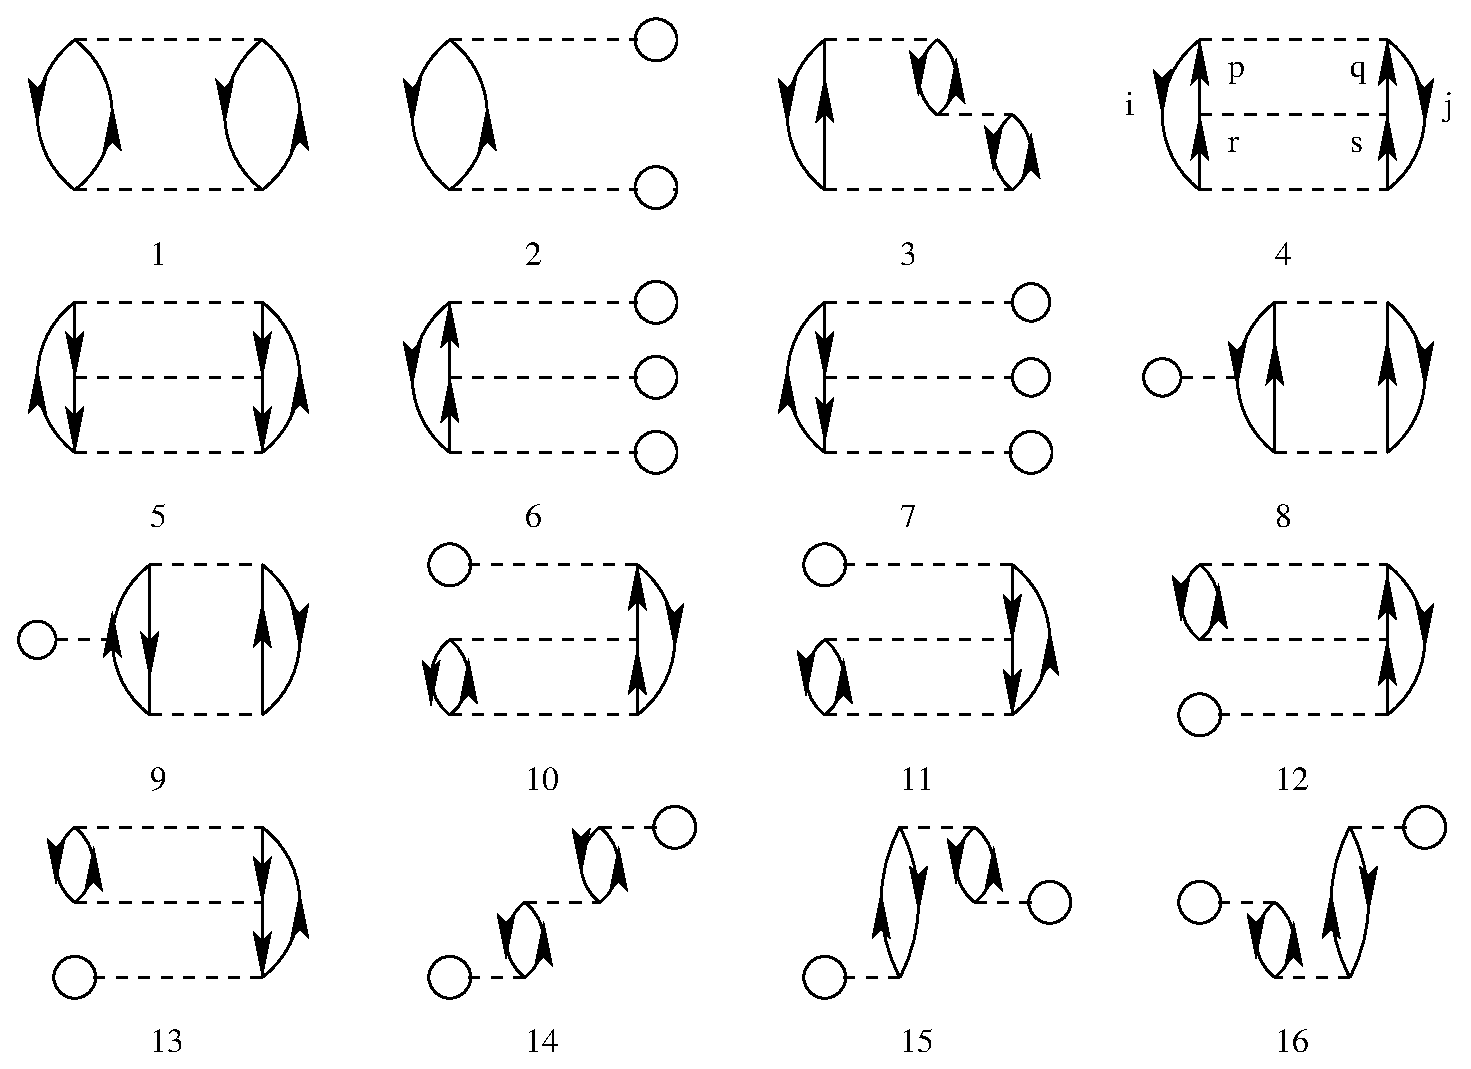
\includegraphics[width=.6\textwidth]{diagrams.eps}
\caption{Diagrams to third order in the interaction. The first order term is excluded.\label{fig:diagrams}}
\end{figure}

Based on the form of the interaction, which diagrams contribute to the binding energy of the ground state?
Write down the expressions for the diagrams that contribute and find the contribution to the ground state
energy as function $g\in [-1,1]$. Comment your results.  Compare these results with those you obtained
in 2) and 3).
\item[e)] The diagrams with only two single particle states as intermediate states (for example diagrams 1 and 4
in Fig.~\ref{fig:diagrams})
can be summed to infinite order since they can be expressed as a geometric series.
Find this contribution and compare the final energy with the results from 2) and 3). Comment your results. 
You can also perform a resummation of diagrams like diagram 5 with hole lines as intermediate states only between
various vertices. Can you find this result as well? Compare now the final results with the resummed
two-particle and two-hole diagrams with the results from 2) and 3).
 
\item[f)] 
We will now set up the Hartree-Fock equations by varying the coefficients of the 
single-particle functions. The single-particle basis functions
are defined as 
\[
\psi_p  = \sum_{\lambda} C_{p\lambda}\psi_{\lambda}.
\]
where in our case $p=1,2,3,4$ and $\lambda=1,2,3,4$, that is the first four lowest single-particle orbits
of Fig.~\ref{fig:schematic}.
Set up the Hartree-Fock equations for this system by varying the coefficients $C_{p\lambda}$ 
and solve them for values of $g\in [-1,1]$. 
Comment your results and compare with the exact solution. Discuss also which diagrams in Fig.~\ref{fig:diagrams}
that can be affected by a Hartree-Fock basis. Compute the total binding energy using a Hartree-Fock basis and
comment your results. 
\item[g)] To fourth order in perturbation theory we can produce diagrams with so-called four-particle-four-hole
excitations. An example is given in Fig.~\ref{fig:fourthorder}.
\begin{figure}[hbtp]
\includegraphics[width=.4\textwidth]{fig8.ps}
\caption{An example of a fourth-order diagram with an intermediate state involving four-particle-four-hole 
excitations.
\label{fig:fourthorder}}
\end{figure}
Find the contribution to the binding energy of the ground state from this type of contributions and compare with your previous results with and without a Hartree-Fock basis. Discuss in particular the connection with the results for the full diagonalization where Slater determinants involving 
four-particle-four-hole excitations are involved.
\item[h)] When summing over all intermediate states in diagram 1 or 4 of Fig.~\ref{fig:diagrams}, we have limited
the sum over intermediate particle states to include the states $p=3$ and $p=4$ only. Compute this sum by taking the limit $p=\infty$. Comment your results.
\end{enumerate}

\subsection*{Exercise 32}
We will study a schematic model (the Lipkin model, Nucl.
Phys. {\bf 62} (1965) 188) for the interaction among  $4$
fermions that can occupy two different energy levels. Each levels has degeneration $d=4$. The two levels have quantum numbers $\sigma=\pm 1$,
with the upper level having  $\sigma=+1$ and energy
$\varepsilon_{1}=
\varepsilon/2$. The lower level  has $\sigma=-1$ and energy
$\varepsilon_{2}=-\varepsilon/2$. 
In addition, the substates  of each level are characterized  
by the quantum numbers $p=1,2,3,4$.

We define the single-particle states
\[
\ket{u_{\sigma =-1,p}}=a_{-p}^{\dagger}\ket{0}
\hspace{1cm}
\ket{u_{\sigma =1,p}}=a_{+p}^{\dagger}\ket{0}.
\]
The single-particle states span an orthonormal basis.
The Hamiltonian of the system is given by
\[
\begin{array}{ll}
H=&H_{0}+H_{1}+H_{2}\\
&\\
H_{0}=&\frac{1}{2}\varepsilon\sum_{\sigma ,p}\sigma
a_{\sigma,p}^{\dagger}a_{\sigma ,p}\\
&\\
H_{1}=&\frac{1}{2}V\sum_{\sigma ,p,p'}
a_{\sigma,p}^{\dagger}a_{\sigma ,p'}^{\dagger}
a_{-\sigma ,p'}a_{-\sigma ,p}\\
&\\
H_{2}=&\frac{1}{2}W\sum_{\sigma ,p,p'}
a_{\sigma,p}^{\dagger}a_{-\sigma ,p'}^{\dagger}
a_{\sigma ,p'}a_{-\sigma ,p}\\
&\\
\end{array}
\]
where $V$ and $W$ are constants. The operator 
$H_{1}$ can move pairs of fermions as shown in Fig.~(a)
while $H_{2}$ is a spin-exchange term.
As shown in Fig.~(b),
$H_{2}$ moves a pair of fermions from a state $(p\sigma ,p' -\sigma)$ to a state
$(p-\sigma ,p'\sigma)$.
\begin{figure}[hbtp]
\includegraphics[width=.4\textwidth]{fig1.ps}
\end{figure}\newline
a) Introduce the quasispin operators
\[
\begin{array}{ll}
J_{+}=&\sum_{p}
a_{p+}^{\dagger}a_{p-}\\
&\\
J_{-}=&\sum_{p}
a_{p-}^{\dagger}a_{p+}\\
&\\
J_{z}=&\frac{1}{2}\sum_{p\sigma}\sigma
a_{p\sigma}^{\dagger}a_{p\sigma}\\
&\\
J^{2}=&J_{+}J_{-}+J_{z}^{2}-J_{z}\\
&\\
\end{array}
\]
Show that these operators obey the commutation relations for angular momentum.\newline
b) Express $H$ in terms of the above quasispin operators and the number operator
\[
N=\sum_{p\sigma}
a_{p\sigma}^{\dagger}a_{p\sigma}.
\]
c) Show that $H$ commutes with $J^{2}$, viz., $J$ is a good quantum number.\newline
d) Consider thereafter a state with all four fermions in the lowest level (see the above figure).
We can write this state as
\[
\ket{\Phi_{J_z=-2}} =a_{1-}^{\dagger}a_{2-}^{\dagger}
a_{3-}^{\dagger}a_{4-}^{\dagger}\ket{0}.
\]
This state has $J_{z}=-2$ and belongs to the set of possible projections of 
$J=2$. We introduce the shorthand notation
$\ket{J,J_z}$ for states with different values of
spin $J$ and its projection $J_z$.

The other possible values are  $J_{z}=-1$, $J_{z}=0$, $J_{z}=1$
and $J_{z}=2$. 
Use the ladder operators
$J_{+}$ and $J_{-}$  to set up the states 
with spin $J_{z}=-1$ $J_{z}=0$, $J_{z}=1$
and $J_{z}=2$.  
The action of these operators on a state with given spin 
$J$ and $J_z$ is  (with $\hbar = 1$) 
$J_+\ket{J,J_z}=\sqrt{J(J+1)-J_z(J_z+1)}\ket{J,J_z+1}$ and
$J_-\ket{J,J_z}=\sqrt{J(J+1)-J_z(J_z-1)}\ket{J,J_z-1}$, respectively.
\newline
e) use thereafter the quasispin operators to construct the Hamiltonian matrix 
$H$ for this five-dimensional space.  Find thereafter the eigenvalues
(numerically using for example Octave or Matlab or python)  for the following parameter sets:
sett av verdier:
\[
\begin{array}{cccc}
(1)&\varepsilon=2,&V=-1/3,&W=-1/4\\
(2)&\varepsilon=2,&V=-4/3,&W=-1
\end{array}
\]
Which state is the ground state? Comment your results.\newline
f)
The single-particle states for the 
 Lipkin model
\[
\ket{u_{\sigma =-1,p}}=a_{-p}^{\dagger}\ket{0}
\hspace{1cm}
\ket{u_{\sigma =1,p}}=a_{+p}^{\dagger}\ket{0}
\]
can now be used as basis for a new single-particle state
$\ket{\phi_{\alpha ,p}}$  via a unitary  transformation
\[
\ket{\phi_{\alpha ,p}}=
\sum_{\sigma =\pm1}C_{\alpha\sigma}\ket{u_{\sigma ,p}}
\]
with $\alpha=\pm 1$ og $p=1,2,3,4$. Why is $p$ the same in 
$\ket{\phi}$
as in $\ket{u}$?  Show that the new basis is orthonormal.\newline
g) With the new basis we can construct a new Slater determinant given by
$\ket{\Psi}$
\[
\ket{\Psi}=\prod_{p=1}^{4}b_{\alpha ,p}^{\dagger}\ket{0}
\]
with $b_{\alpha ,p}^{\dagger}\ket{0}=\ket{\phi_{\alpha ,p}}$.
h)   Use the Slater determinanten from the previous exercise to calculate
\[
E=\bra{\Psi}H\ket{\Psi},
\]
as a function of the coefficients $C_{\sigma\alpha}$. We assume the coefficients to be real.\newline
i) Show that
\[
  \frac{\epsilon}{3} > V+W,
\]
has to be fulfilled in order to find a minimum in the energy.

Hint: calculate the functional derivative  of the energy with respect to the coefficients $C_{\sigma\alpha}$. 

\subsection*{Exercise 33, Exam Fall semester 2011}
Let $\hat{H}=\hat{H}_0 +\hat{H}_I$ and $\ket{\Phi_n}$ be the eigenstates of $\hat{H}_0$ and that
$\ket{\Psi_n}$ are the corresponding ones for $\hat{H}$. 
Assume that the ground states
$\ket{\Phi_0}$ and $\ket{\Psi_0}$ are not degenerate. 
We can then write the energy of the ground state as
\[
E_0 -\varepsilon_0 =\frac{\bra{\Phi_0} \hat{H}_I\ket{\Psi_0}}
{\left\langle \Phi_0 | \Psi_0 \right\rangle},
\]
with $\hat{H}\ket{\Psi_0} =E_0\ket{\Psi_0}$ and
$H_0\ket{\Phi_0} =\varepsilon_0\ket{\Phi_0}$. We 
define also the projection operators $\hat{P}=\ket{\Phi_0}\bra{\Phi_0}$ and $\hat{Q}=1-\hat{P}$. 
These operators satisfy $\hat{P}^2=\hat{P}$, $\hat{Q}^2=\hat{Q}$ and $\hat{P}\hat{Q}=0$.
\begin{enumerate}
\item[a)]
Show that for any  $\omega$ we have can write the ground state energy as
\[
E_0=\varepsilon_0+
    \sum_{n=0}^{\infty}\bra{\Phi_0}\hat{H}_I
    \left(\frac{\hat{Q}}{\omega-\hat{H}_0}(\omega-E_0+\hat{H}_I)\right)^n
    \ket{\Phi_0}.
\]
\item[b)]
Discuss these results  for $\omega=E_0$ (Brillouin-Wigner perturbation theory)
and $\omega=\varepsilon_0$ (Rayleigh-Schr\"{o}dinger perturbation theory).
Compare the first few terms in these expansions and discuss the differences.
\item[c)] Show that the onebody part of the Hamiltonian
    \[
        \hat{H}_0 = \sum_{pq} \element{p}{\hat{h}_0}{q} a^\dagger_p a_q
    \]
can be written, using standard annihilation and creation operators, in normal-ordered form as 
    \[
        \hat{H}_0 = \sum_{pq} \element{p}{\hat{h}_0}{q} a^\dagger_p a_q=\sum_{pq} \element{p}{\hat{h}_0}{q} \left\{a^\dagger_p a_q\right\} +
                \sum_i \element{i}{\hat{h}_0}{i}, \]
and that the two-body Hamiltonian 
    \[
        \hat{H}_I = \frac{1}{4} \sum_{pqrs} \element{pq}{\hat{v}}{rs} a^\dagger_p a^\dagger_q a_s  a_r,
    \]
can be written 
\[
\hat{H}_I=\frac{1}{4} \sum_{pqrs} \element{pq}{\hat{v}}{rs} \normord{a^\dagger_p a^\dagger_q a_s  a_r}
            + \sum_{pqi} \element{pi}{\hat{v}}{qi} \normord{a^\dagger_p a_q} + \frac{1}{2} \sum_{ij} \element{ij}{\hat{v}}{ij}
\]
Explain the meaning of the various symbols. Which reference 
vacuum has been used?  Write down the diagrammatic representation of all these terms. 
\item[d)]  Use the diagrammatic representation of the Hamiltonian operator 
from the previous exercise to set up all diagrams (use either 
anti-symmetrized Goldstone diagrams or Hugenholz diagrams)
to second order (including the reference energy) in Rayleigh Schr\"odinger perturbation theory 
that contribute to the expectation value of $E_0$.

Use the diagram rules to write down their closed-form expressions.
If a Hartree-Fock basis is used, which diagrams remain?
\end{enumerate}
We consider now a one-particle system with the following Hamiltonian
$\hat{H}=\hat{H}_{0}+\hat{H}_{I}$ where
\[
\hat{H}_{0}=\sum_{p}\varepsilon_{p}a_{p}^{\dagger}a_{p},
\]
and
\[
\hat{H}_{I}=g\sum_{pq}a_{p}^{\dagger}a_{q}.
\]
The strength parameter $g$ is a real constant.  
The first part of the Hamiltonian plays the role of the unperturbed part,
with 
\[
\element{p}{\hat{h}_0}{q}=\delta_{p,q}\varepsilon_{p}.
\]
We have only two one-particle states, with $\varepsilon_{1}< \varepsilon_{2}$, and we will let the first state $p=1$ correspond to the
model space and the other, $p=2$, correspond to the excluded space.  Use labels $ijk\dots$ for hole
states (below the Fermi level) and labels $abc\dots$ for particle (virtual) 
states (above the Fermi level).
\begin{enumerate}
\item[e)] Use the results from exercise c) to write down the above  Hamiltonian 
in a normal-ordered form and set up all diagrams.  Use an $X$  to indicate the interaction part $H_I$.
\item[f)] Define the ground state (which is our model space) as 
\[
\ket{\Phi_0}=a_{i}^{\dagger}\ket{0}=a_{1}^{\dagger}\ket{0},
\]
and the excited state as
\[
\ket{\Phi_i^a}=a_{a}^{\dagger}a_i\ket{\Phi_0},
\]
where $a=2$ and $i=1$.  Set up the Hamiltonian matrix (a $2\times 2$ matrix) and find the 
exact energy 
and expand the exact result for the ground state in terms of the
parameter $g$.  
\item[g)] Find the ground state energy to third order in Rayleigh-Sch\"{o}dinger 
perturbation theory and compare the results with the expansion of the exact energy from the previous exercise. Write down all diagrams which contribute and comment your results.
\end{enumerate}
The final part deals with coupled-cluster theory. Since we have only a one-body problem,
coupled-cluster theory truncated at the level of $T_1$  is exact.  The similarity transformed 
normal-ordered Hamiltonian can then be written out as
   \[
        \bar{H} = \hat{H}_N + \left( \hat{H}_N \hat{T}\right)_c + \frac{1}{2} \left( 
\hat{H}_N \hat{T}^2\right)_c
            + \dots +,
    \]
where only linked diagrams appear.
The expectation value of the ground state energy (beyond the reference energy is) 
\[
        \mathrm{E}_{\mathrm{CCS}} = \bra{\Phi_0} \bar{H} \ket{\Phi_0},
 \]
and the amplitudes $t_i^a$ are determined from the equation
\[
        0 = \bra{\Phi_i^a} \bar{H} \ket{\Phi_0}.
\]
For the latter we need to take into account diagrams which lead to a final excitation level of
$+1$ only.
\begin{enumerate}
\item[h)] Set up the definition of the operator $\hat{T}=\hat{T}_1$.  We will use a diagrammatic approach only  to find the diagrammatic contribution to the ground state beyond the reference energy. Show
that the only possibility is  
\[
    E_{CCS} = 
    \parbox{15mm}{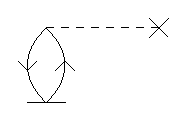
\includegraphics[scale=0.5]{graphics/ccsd_e1}}
\]
Find the closed form expression. 
\item[i)]
Show, using a diagrammatic approach and keeping in mind the final excitation level,  
that the only diagrams that lead to 
\[
        0 = \bra{\Phi_i^a} \bar{H} \ket{\Phi_0},
\]
are
\[
    0=\parbox{10mm}{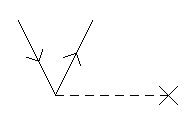
\includegraphics[scale=0.4]{graphics/ccsd_hbar_04a}}
    + \parbox{18mm}{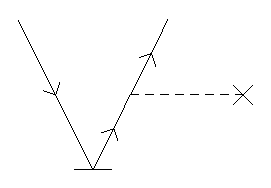
\includegraphics[scale=0.4]{graphics/ccsd_hbar_04b}}
    + \parbox{15mm}{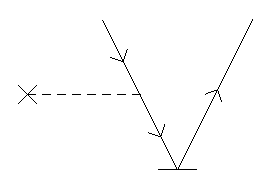
\includegraphics[scale=0.4]{graphics/ccsd_hbar_04c}}
    + \parbox{15mm}{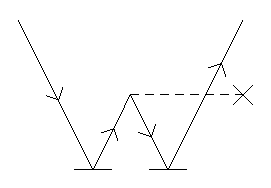
\includegraphics[scale=0.4]{graphics/ccsd_hbar_04h}} \\
\]
Set up the final closed form expressions and the algorithm for finding the amplitudes $t_i^a$. 
Can you solve the problem? 
\end{enumerate}

\end{document}
